\graphicspath{ {Implementation/Images/} }


\chapter{Word2Vec Model Building}
\label{cha:implementation}

\section{Introduction}
In this chapter 

DiseaseMapping (generalization)
OSIM
Clusters
TensorFlow
DL4J

\section{OSIM2 Dataset}
\label{sec:osim2DS}

To validate our approaches mentioned in section \ref{sec:gw2v}, we rely on the Observational Medical Dataset Simulator Generation 2 (OSIM2) dataset \cite{OSIM:online}. This dataset was generated by the Observational Medical Outcomes Partnership (OMOP) as a golden standard to be able to reproduce studies about the effects of drug treatments. It contains around $10$ million of hypothetical patients based on Thomson Reuters MarketScan Lab Database (MSLR). MSLR contains administrative claims between 2003 and 2009 from a privately-insured population. There are $16$ different OSIM2 datasets where each of them is injected with different kinds of signals. We rely on the "OSIM2\_10M\_MSLR\_MEDDRA\_14". \\

The OSIM2 dataset contains multiple database tables which are dumped as comma-separated values (csv) files. The files contain information about the patients' demographics, diagnoses, drug treatments, timestamps, hospital visits, \ldots \\
To make it easier to work with this dataset, we joined the multiple files into one file with on each row an event of a patient containing all relevant information. The relevant information which is kept is: birth year, gender, condition type, condition (MedDRA coding), time difference since previous diagnosis, and season (summer, fall, winter, spring). We ignored drug treatments and hospital visits as those are too complex to categorize. Thus, one EHR event (or vector $m$) is $6$ dimensional, see table \ref{tab:general} for an example. \\	

We will compare our model with the clusters found in Anders Boeck Jensen et. \cite{Brunak:article} (see section \ref{sec:brunak}). Although these clusters are not a golden standard, it is the only study to which we can compare our model. It provides an initial idea on how well our model estimates disease relations. In section \ref{sec:PatientClassification}, we introduce a validation approach which can be explored in the future. \\
Before we can compare our model to the clusters found in the Danish paper, we have to apply several estimations and methods which are described in section \ref{sec:convertionClusters}.


\section{Software Ecosystem}

To build our model, we look for a software library which provides us with the following tools:

\begin{itemize}

\item Word2Vec implementation
\item Highly customizable as we want to adjust internal workings of Word2Vec
\item Built with large datasets in mind (no memory leaks, multi-threading)

\end{itemize}

\subsection{TensorFlow}

TensorFlow is an open-source machine learning software library released at the end of 2015 \cite{tensorflow:article}. It is developed by the Google Brain Team. It puts its focus on neural networks and their applications in language processing and image recognition. \\
It provides a Python interface for efficient C++ code. We found that Tensorflow is not well documented and does not provide the freedom needed to easily rewrite some core features of the Word2Vec implementation, for example manipulating the internal trained lookup table to add new instances based on knn.


\subsection{DeepLearning4Java}

DeepLearning4Java (DL4J) is an open-source machine learning software library released by Skymind \cite{dl4j:article}. It puts its focus on deeplearning and makes it possible to easily extend DL4J's implementation with the user's implementation. \\
It runs on their scientific computing engine ND4J which provides fast matrix operations. DL4J is completely written in Java and provides a lot of freedom to manipulate lookup tables and extend Word2Vec methods to work on abstract objects such as vectors.


\section{Generalized Word2Vec Model Building}
\label{sec:convertionClusters}

As described in section \ref{sec:gw2v}, we use generalized Word2Vec approaches to find patterns in EHR data. We use the OSIM2 dataset and represent each EHR event as a $6$ dimensional vector. This vector is comparable to a word in a normal Word2Vec approach and functions as the abstract object in our generalized Word2Vec approaches. 

\subsection{Categorization of Features}
\label{sec:categorizationImpl}

Because we are working with high dimensional data and a each dimension has a wide range of possible values, most instances of OSIM2 are unique. To find patterns which are more generally applicable, we generalize our data by projecting values for some attributes into categories. See table \ref{tab:catOsim}. \\

\begin{table}[!htb]
\centering
\begin{tabular}{lll}
\hline
Attribute                                    & Requirement                      & Category \\ \hline
\multicolumn{1}{l|}{Time between EHR events} & \multicolumn{1}{l|}{$\leq 0$}    & 0        \\
\multicolumn{1}{l|}{}                        & \multicolumn{1}{l|}{$\leq 10$}   & 1        \\
\multicolumn{1}{l|}{}                        & \multicolumn{1}{l|}{$\leq 20$}   & 2        \\
\multicolumn{1}{l|}{}                        & \multicolumn{1}{l|}{$20 <$}      & 3        \\ \hline
\multicolumn{1}{l|}{Birthyear}               & \multicolumn{1}{l|}{$\leq 1900$} & 0        \\
\multicolumn{1}{l|}{}                        & \multicolumn{1}{l|}{$\leq 1910$} & 1        \\
\multicolumn{1}{l|}{}                        & \multicolumn{1}{l|}{$\leq 1920$} & 2        \\
\multicolumn{1}{l|}{}                        & \multicolumn{1}{l|}{\vdots}      & \vdots   \\
\multicolumn{1}{l|}{}                        & \multicolumn{1}{l|}{$\leq 2020$} & 12       \\ \hline
\multicolumn{1}{l|}{Season}                  & \multicolumn{1}{l|}{}            & 3 (winter) \\
\multicolumn{1}{l|}{}                        & \multicolumn{1}{l|}{}            & 4 (spring)   \\
\multicolumn{1}{l|}{}                        & \multicolumn{1}{l|}{}            & 1 (summer)   \\
\multicolumn{1}{l|}{}                        & \multicolumn{1}{l|}{}            & 2 (fall)    \\ \hline
\end{tabular}

\caption{Different categories for OSIM2 attributes.}
\label{tab:catOsim}
\end{table}

It is easy to generalize concepts such as time intervals and demographics, for example we can say that people between the age $0$ and $10$ belong to category A. This becomes complex for disease diagnoses as it requires a lot of knowledge to categorize those. We come back to disease coding in section \ref{sec:mapping}. \\

To see the effect of our categorizations, see table \ref{tab:general}. You can see the $3$ most common vectors from our dataset before and after the categorizations. The vectors have the following structure: \textit{{[}birthyear, gender, conditionType, diagnose, timeDifference, season{]}}. \\

\begin{table}[!htb]
\centering

\begin{tabular}{lll}
\hline
\textbf{Before Categorization}                                                    &                             &                     \\ \hline
\textit{Vector} & \textit{Occurrences}        & \textit{Percentage} \\ \hline
\multicolumn{1}{l|}{{[}1956.0, 8532.0, 65.0, 5.00000701E8, 0.0, 3.0{]}}           & \multicolumn{1}{l|}{17574}  & 0.0095              \\
\multicolumn{1}{l|}{{[}1954.0, 8532.0, 65.0, 5.00000701E8, 0.0, 3.0{]}}           & \multicolumn{1}{l|}{17536}  & 0.0094              \\
\multicolumn{1}{l|}{{[}1955.0, 8532.0, 65.0, 5.00000701E8, 0.0, 3.0{]}}           & \multicolumn{1}{l|}{17476}  & 0.0094              \\
                                                                                  &                             &                     \\ \hline
\textbf{After Categorization}                                                     &                             &                     \\ \hline
\textit{Vector} & \textit{Occurrences}        & \textit{Percentage} \\ \hline
\multicolumn{1}{l|}{{[}6.0, 8532.0, 65.0, 784955.0, 1.0, 3.0{]}}                  & \multicolumn{1}{l|}{282086} & 0.15                \\
\multicolumn{1}{l|}{{[}7.0, 8532.0, 65.0, 784955.0, 1.0, 3.0{]}}                  & \multicolumn{1}{l|}{235459} & 0.13                \\
\multicolumn{1}{l|}{{[}5.0, 8532.0, 65.0, 784955.0, 1.0, 3.0{]}}                  & \multicolumn{1}{l|}{230216} & 0.12               
\end{tabular}

\caption{Three most common vectors in our dataset before and after categorization.}
\label{tab:general}
\end{table}


\subsection{Disease Code Categorization and Mapping}
\label{sec:mapping}

In the section we discuss the method to categorize the disease codes in the OSIM2 dataset.  For example, a bruise on your right leg and a bruise on your left leg should both be categorized under a bruises category. \\

The OSIM2 dataset uses MedDRA disease codes for the diagnoses, see section \ref{sec:diseaseCodes}. We mentioned that MedDRA does not have an easy to use hierarchy. With a hierarchy, it would be trivial to categorize a disease code to its highest hierarchy. \\
To solve this, we map MedDRA disease codes to ICD-10 disease codes. The reasoning behind this is that ICD-10 provides a clear and easy to use hierarchy. Next to this, ICD-10 disease codes also make it possible to compare our results with \cite{Brunak:article}. \\
We would have liked to use the method described in \cite{icd10Mapping:article} to map the codes but therefore the disease mapping made by UMLS between ICD-10 and MedDRA is needed. This however is not publicly available. \\

The mapping is based on the description of each disease code. Both MedDRA and ICD-10 have a short medical description of each code. Each description is first filtered from stop words. Afterwards, the MedDRA code is matched to the ICD-10 code based on the matching words in both descriptions. The matching is defined as the ICD-10 code with the highest percentage of words matching. \\

In figure \ref{fig:mappingStats}, we show the statistics of this mapping process. Note that we only take disease codes into account if they are part of the OSIM2 dataset. In the figure, each bar represents the percentage of the words matching between descriptions. The height of the bars represent the percentage of all disease codes in the OSIM2 dataset which have this amount of word matches. \\

\begin{figure}[!htb]
	\centering
	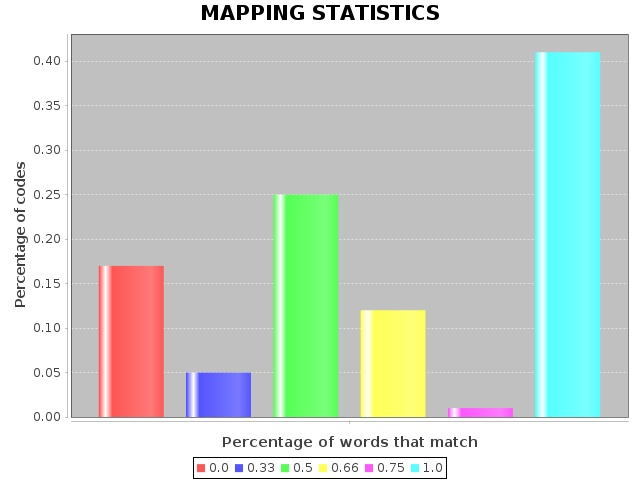
\includegraphics[width=0.7\textwidth]{mappingStats.jpeg}
	\caption{Percentage of OSIM codes compared to their fraction of their matching words.}
	\label{fig:mappingStats}
\end{figure}

We find a $63$\% average of the words in the description that match between MedDRA and ICD-10 descriptions. We also see that around $85$\% of all the disease code mappings have a match of at least $33$\%. We assume this is a reasonable mapping as medical terms are quite specific and if $33$\% matches, this corresponds to a match on to a higher hierarchical level. \\
For the codes which have a zero percent match, the Damerau-Levenshtein algorithm \cite{edit:article} is applied. The algorithm calculates the edit distance between two strings using character insertion, character deletion, character replacement, and adjacent character swaps. The description with the lowest edit distance is then chosen as a match. \\
Another option would have been to remove those codes from our dataset. As an EHR contains more information than only the disease code, a lot of information would have been lost. This however is not tested and is a possibility for future work. \\

With the mapping, we can now categorize the disease codes. We use the hierarchy of ICD-10 and reduce the ICD-10 code to its first $3$ symbols. For example, we reduce the code \textit{E00.1} to its higher category \textit{E00}.


\subsection{Comparison with Danish Clusters}
\label{sec:clusterExp}

To test our approaches we compare our results with the clusters found from Anders Boeck Jensen et. \cite{Brunak:article}, we call these the Danish clusters. For this, we first need to generate our own clusters from OSIM2. This method is described in this section. Note that the comparison with the Danish paper is not ideal as mentioned in section \ref{sec:osim2DS}. We refer to chapter \ref{cha:futureWork} for information about another possible experiment in the future. \\

We now explain how we construct clusters from OSIM2 based on our Word2Vec model, we call these Word2Vec clusters. Afterwards, we compare the Word2Vec clusters with the Danish cluster and define a matching percentage between the two. \\

First we apply our generalized Word2Vec approaches on the OSIM2 dataset. For a description of the parameters used and their functions, see section \ref{sec:parameters}. As end result, we obtain a lookup table containing the mapping between the old vector space and the new one. From this lookup table, we take EHR events and find their k-nearest neighbors from the other events in the new vector space (see section \ref{sec:parameters} for more information about clusterK). The Word2Vec clusters are the set of the EHR event and its knn. \\
Depending on the approach, we take all or a subset of the EHRs. \\

We now describe $2$ experiments which find a matching percentage between the two kinds of clusters. \\
The first experiment goes as follows:

\begin{itemize}

\item We start with an element $e_{wv}$ from the lookup table and form a Word2Vec cluster $C_{wv}$ around it as described above.
\item We then check to which Danish cluster $C_d$ element $e_{wv}$ belongs.
\item For each element in $C_{wv}$, we check if it belongs to $C_d$.
\begin{itemize}
\item If it does, we add $1$ to the number $t_{matches}$.
\item If it does not, we add $1$ to the number $t_{non\_matches}$.
\end{itemize}
\item After doing this for all elements in $C_{wv}$, we calculate the matching percentage as $p_{match} = \frac{t\_{matches}}{t_{matches} + t_{non\_matches}} = \frac{t\_{matches}}{\left| C_{wv} \right|}$.

\end{itemize}

\noindent The second experiment goes as follows:

\begin{itemize}

\item We start with an element $e_{wv}$ from the lookup table and form a Word2Vec cluster $C_{wv}$ around it as described above.
\item We then check to which Danish cluster $C_d$ element $e_{wv}$ belongs.
\item We set $t_{d}$ equals to the number of elements in $C_d$.
\item For each element in $C_{wv}$, we check if it belongs to $C_d$.
\begin{itemize}
\item If it does, we add $1$ to the number $t_{matches}$.
\end{itemize}
\item After doing this for all elements in $C_{wv}$, we calculate the match percentage as $p_{match} = \frac{t\_{matches}}{t_{d}} = \frac{t\_{matches}}{\left| C_{d} \right|}$.

\end{itemize}

For each method, we calculate the average $p_{match}$ over all elements in the lookup table and keep track of the maximum and minimum value for $p_{match}$.


\subsection{Parameters}
\label{sec:parameters}

The effectiveness of a neural network such as the one used to learn disease embeddings, depends on parameter tuning. Parameter tuning is a difficult problem and complex methods have been proposed to solve this \cite{tuning:article}. Therefore we explored $504$ different settings. Note that this is not an extensive parameter tuning setup, but an overview on the effect and logic behind some parameters. An extensive parameter tuning setup is possible as future work. \\

In table \ref{tab:parameters}, you can see an overview of the different parameters for each approach. Every time, all possible combinations of the mentioned parameters have been tested. \\
To our knowledge, there is only one study about the tuning of Word2Vec parameters \cite{w2vTuning:article}. In this study they start with picking some values for the parameters and do an extensive study on which value performs best. We take a similar approach by choosing some values and see their effects. Another iteration should be executed to tune our Word2Vec approaches better by taking our findings into account from our results described in section \ref{sec:expResults}. This is a possible road to explore in future work. \\

\begin{table}[!htb]
\centering

\begin{tabular}{llll}
\hline
Parameter                                    & Generalized Word2Vec  & Knn Word2Vec          & DeepWalk              \\ \hline
\multicolumn{1}{l|}{Vectorlength}            & {[}50, 100{]}         & {[}50, 100{]}         & {[}50, 100{]}         \\
\multicolumn{1}{l|}{Batch Size}              & 500                   & 500                   & 500                   \\
\multicolumn{1}{l|}{Epoch}                   & 1                     & 1                     & 1                     \\
\multicolumn{1}{l|}{Window Size}             & {[}5, 10, 15{]}       & {[}5, 10, 15{]}       & {[}5, 10, 15{]}       \\
\multicolumn{1}{l|}{Learning Rate}           & {[}0.025, 0.1{]}      & {[}0.025, 0.1{]}      & {[}0.025, 0.1{]}      \\
\multicolumn{1}{l|}{Minimum Word Frequency} & {[}5, 10{]}           & {[}5, 10{]}           & {[}5, 10{]}           \\
\multicolumn{1}{l|}{ClusterK}                & {[}100, 1000, 5000{]} & {[}100, 1000, 5000{]} & {[}100, 1000, 5000{]} \\
\multicolumn{1}{l|}{K}                       & /                     & {[}10, 50, 100{]}     & /                     \\
\multicolumn{1}{l|}{Walklength}              & /                     & /                     & {[}5, 10, 15{]}      
\end{tabular}

\caption{Parameters which are tested for the different approaches}
\label{tab:parameters}
\end{table}

\noindent\textbf{Vectorlength} fixes the dimensions of the new vector space to which the EHR events are projected to. A larger size is more expressive but a smaller size decreases the complexity of the vocabulary after training. Each dimension can be seen as a representation of an unknown linear relation to some context-disease pairs \cite{vl:article}. \\
\textbf{Batch size} is the number of training examples used in one gradient descent step. \\
\textbf{Epoch} is the number of times you go over all the training examples and use them to train your neural network by updating the weights. \\
\textbf{Window size} is the size of the n-gram we use to create contexts. A window size is an estimation of the relevant context for a word. This means that the window size depends on the used corpus \cite{w2vOriginal:article} \cite{windowSize:article}. \\
\textbf{Learning rate} decides how the weights are adjusted during backpropagation. A large value makes the neural network learn faster but may also cause the network not to learn at all. A small value on the other hand can cause a slow convergence or overfitting \cite{lr:article}. \\
Note that in our implementation, we use an adaptive gradient (AdaGrad) descent algorithm \cite{adagrad:article}. Informally, it increases the learning rate for sparse features and therefore is able to take predictive but rarely seen features into account.  \\
\textbf{Minimum Word Frequency} removes instances from the training set below a certain minimum value. A low frequency causes the inclusion of instances which only have a few contexts for which relations can be learned from. A higher frequency could improve the accuracy for a Word2Vec model but also throw away information. Note that the influence of this parameter is not well researched. \\
\textbf{ClusterK} is the parameter which creates Word2Vec clusters as described in the previous section. A higher clusterK causes the Word2Vec cluster to be larger and a lower value the other way around. \\
\textbf{K} is a specific parameter for the knn Word2Vec approach. It decides on how many nearest neighbors the new vector representation is based on. For more explanation see section \ref{sec:knnWord2Vec}. \\
\textbf{Walklength} is a specific parameter for DeepWalk. It decides how long the generated sequence will be. For more explanation see section \ref{sec:deepwalk}.

\section{Results}
\label{sec:expResults}

Here we discuss the results from our two experiments on the generalized Word2Vec approaches. We compare the Word2Vec clusters with the Danish cluster as described in section \ref{sec:clusterExp}. \\
We check the influence of a parameter on the matching percentage by inspecting each parameter setting. From all these parameter settings, we deduce a general trend on the influence of the studied parameter. \\
After checking the individual parameters, we take the parameter setting with the highest average matching percentage for each approach and compare the different approaches. \\

The bars in the figures of this section each show a parameter value and the black stripes both represent the minimum and the maximum value of the matching percentage. The height of each bar represents the matching percentage.

\subsection{Generalized Word2Vec}

We use the complete OSIM2 dataset to make our Word2Vec model and make Word2Vec clusters from all instances in the lookup table. \\
Both in experiment $1$ and experiment $2$, we found that the vectorlength, window size, learning rate, and minimum word frequency have no substantial influence on the matching percentage. 

\subsubsection{Vectorlength}

For the influence of the vectorlengths, see figure \ref{fig:s2v_vl} for the matching percentage of experiment $1$ (left) and experiment $2$ (right). \\

\begin{figure}[!htb]
	\centering
	\begin{subfigure}[b]{.49\textwidth}\
		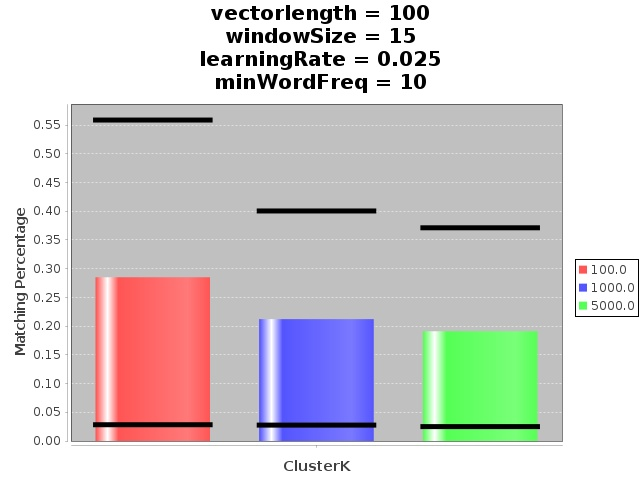
\includegraphics[width=\textwidth]{S2V1_vl.jpeg}
	\end{subfigure}
	\begin{subfigure}[b]{.49\textwidth}
		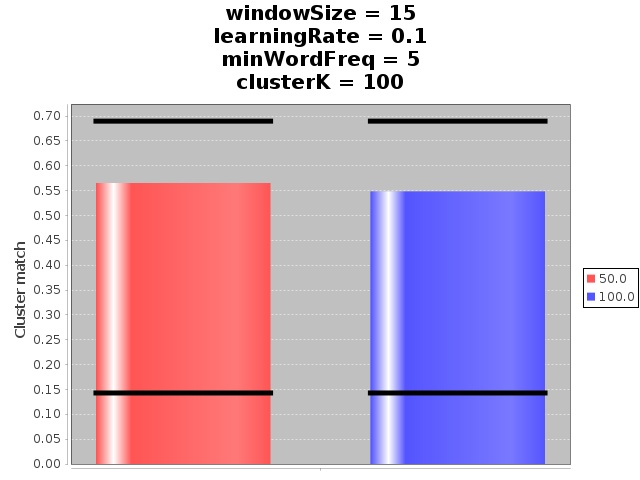
\includegraphics[width=\textwidth]{S2V2_vl.jpeg}
	\end{subfigure}
	\caption{Mapping percentage for different vectorlengths of the generalized Word2Vec 		approach in both experiments.}
	\label{fig:s2v_vl}
\end{figure}

We conclude that a vectorlength of $50$ is expressive enough to differentiate between different diseases of the OSIM2 dataset as it gives the same results as a vectorlength of $100$. Only sometimes the vectorlength of $100$ gives a small gain in matching percentage which can be explained by the increase of expressiveness of the new vector space.

\subsubsection{Window Size}

For the influence of the window sizes, see figure \ref{fig:s2v_vl} for the matching percentage of experiment $1$ (left) and experiment $2$ (right). \\

\begin{figure}[!htb]
	\centering
	\begin{subfigure}[b]{.49\textwidth}\
		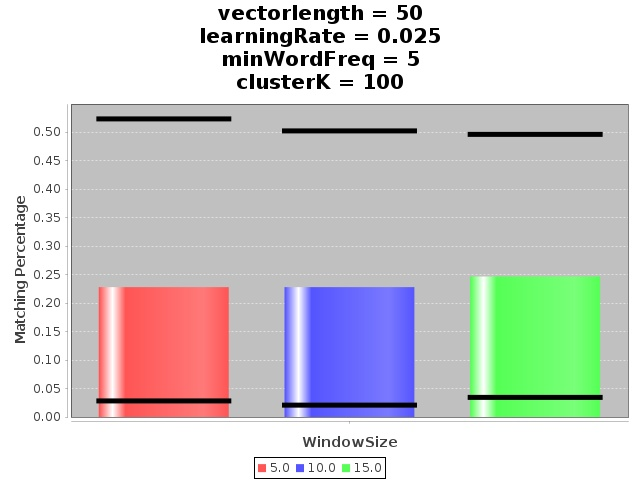
\includegraphics[width=\textwidth]{S2V1_ws.jpeg}
	\end{subfigure}
	\begin{subfigure}[b]{.49\textwidth}
		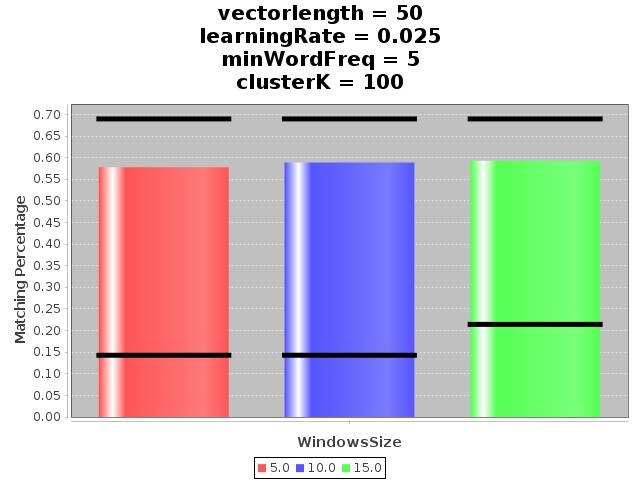
\includegraphics[width=\textwidth]{S2V2_ws.jpeg}
	\end{subfigure}
	\caption{Mapping percentage for different window sizes of the generalized Word2Vec 		approach in both experiments.}
	\label{fig:s2v_ws}
\end{figure}

We expected the window size to have more impact as a higher size makes more specific contexts and therefore we expected a better model. A reason for this negative result can be that we do not have enough data to justify more specific contexts or we did not find a good window size to approximate the relevant contexts for our dataset. \\
Also, because our sequence lengths have an average length of around $19$, a window size of $5$ is not that much different than a size of $10$ as in many cases it will cut of the size at the start or end of the sequence. The Danish paper uses sequences of length $4$, so this could also imply that a window size of $5$ is already enough to cover the relationships the Danish paper found and therefore a higher size will not have an impact on the matching percentage. \\
The Danish paper sets a $5$ year 'window size' as they assume no dependencies are possible between disease outside this time frame. To achieve a similar effect with the window size of Word2Vec, a varying window size should be used. To our knowledge, a varying window size is only tested in \cite{w2vTuning:article} but no clear implementation is given. 

\subsubsection{Learning Rate}

For the influence of the learning rates, see figure \ref{fig:s2v_lr} for the matching percentage of experiment $1$ (left) and experiment $2$ (right). \\

\begin{figure}[!htb]
	\centering
	\begin{subfigure}[b]{.49\textwidth}\
		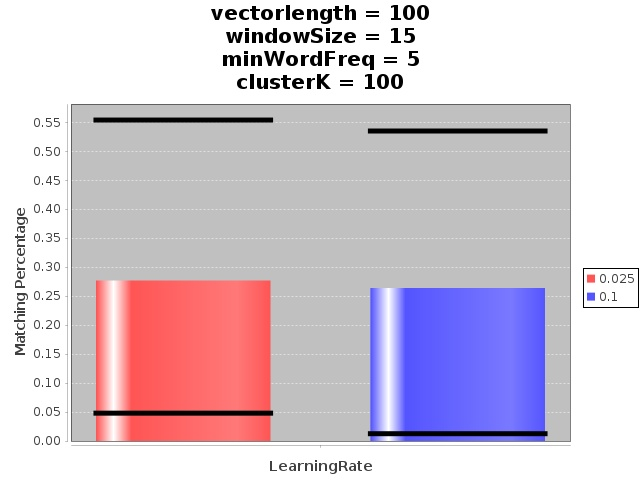
\includegraphics[width=\textwidth]{S2V1_lr.jpeg}
	\end{subfigure}
	\begin{subfigure}[b]{.49\textwidth}
		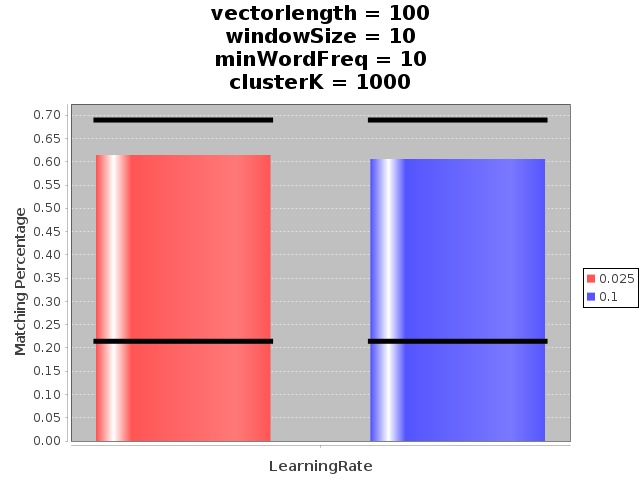
\includegraphics[width=\textwidth]{S2V2_lr.jpeg}
	\end{subfigure}
	\caption{Mapping percentage for different learning rates of the generalized Word2Vec 		approach in both experiments.}
	\label{fig:s2v_lr}
\end{figure}

Learning rate is a parameter which is hard to tune \cite{peskyLr:article}. This explains the amount of literature around learning rate and the implementation of automatic tuning algorithms for learning rate \cite{peskyLr:article} \cite{adagrad:article} \cite{lrHard:article}. Therefore our results do not provide any final conclusion as we only tested $2$ different learning rates which is not extensive enough for a difficult parameter as the learning rate. \\
Although it is also possible that we chose our learning rate similar enough in both cases and because of AdaGrad (see section \ref{sec:parameters}, they both achieved the same results.

\subsubsection{Minimum Word Frequency}

For the influence of the minimum word frequencies, see figure \ref{fig:s2v_wf} for the matching percentage of experiment $1$ (left) and experiment $2$ (right). \\

\begin{figure}[!htb]
	\centering
	\begin{subfigure}[b]{.49\textwidth}\
		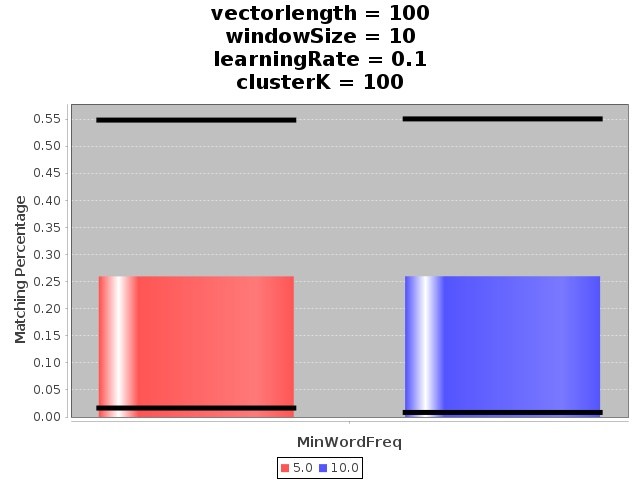
\includegraphics[width=\textwidth]{S2V1_wf.jpeg}
	\end{subfigure}
	\begin{subfigure}[b]{.49\textwidth}
		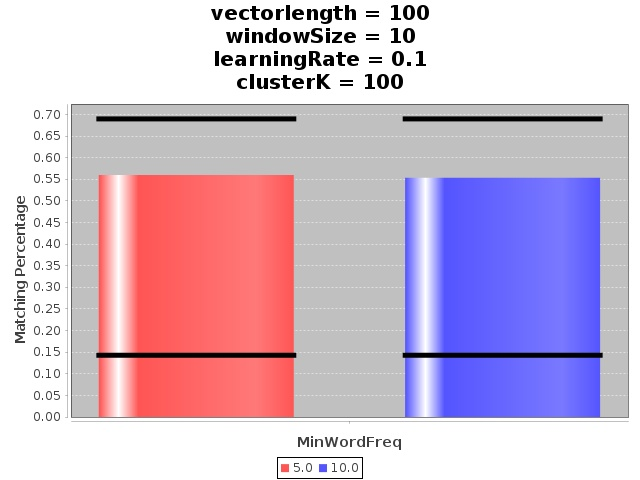
\includegraphics[width=\textwidth]{S2V2_wf.jpeg}
	\end{subfigure}
	\caption{Mapping percentage for different minimum word frequencies of the generalized Word2Vec approach in both experiments.}
	\label{fig:s2v_wf}
\end{figure}

We expected the minimum word frequency to result in a better accuracy for a higher value. Otherwise, some instances will only have a few occurrences which would make it hard to learn from. \\
However, because we applied generalization, $99.82$\% of the instances are above the minimum word frequency of $10$ with respect to $69.90$\% before generalization. We therefore expect the minimum word frequency to have lost its influence. A future direction to explore is to ignore the generalization and solely work with minimum word frequency.

\subsubsection{ClusterK}

See figure \ref{fig:s2v_clusterK_1} for the influence in the matching percentage of experiment $1$ by the parameter clusterK. Similar results are achieved with all the other parameter settings. \\

\begin{figure}[!htb]
	\centering
	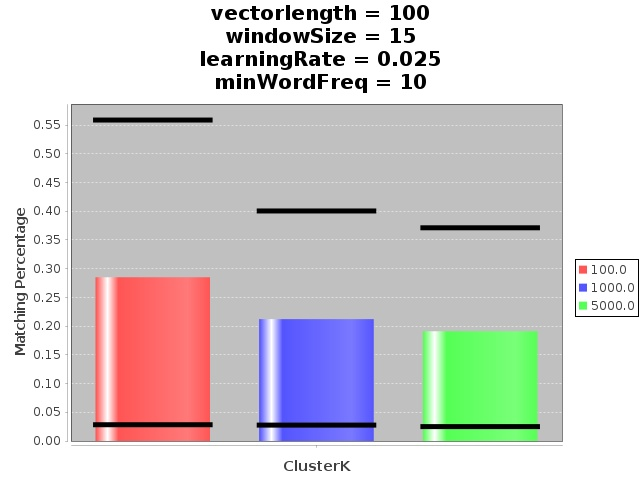
\includegraphics[width=0.6\textwidth]{S2V1_clusterK.jpeg}
	\caption{Mapping percentage for different clusterKs of the generalized Word2Vec approach in experiment $1$.}
	\label{fig:s2v_clusterK_1}
\end{figure}

\noindent We see a trend that with a lower clusterK there is a higher matching percentage. This means that in the smaller clusters, there is a higher density of instances which correspond to the Danish clusters. This shows that our method is not completely random especially in the case of some disease codes as a maximum matching percentage of $55$\% is found. Especially since we used several estimations such as the disease code mapping, different datasets, and categorization. \\

\noindent See figure \ref{fig:s2v_clusterK_2} for the influence in the matching percentage of experiment $2$ by the parameter clusterK. Similar results are achieved with all the other parameter settings. \\

\begin{figure}[!htb]
	\centering
	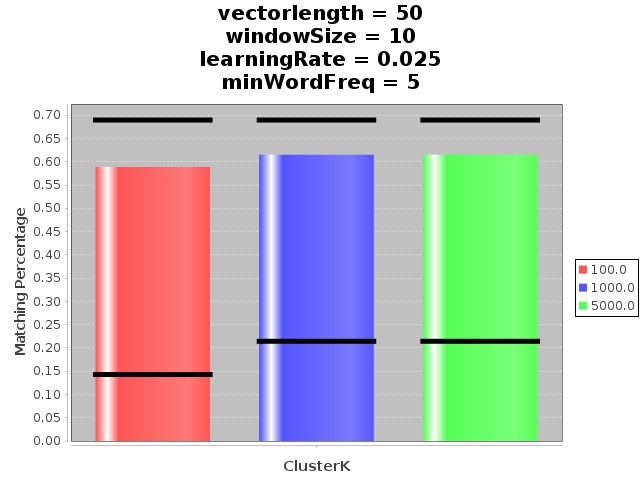
\includegraphics[width=0.6\textwidth]{S2V2_clusterK.jpeg}
	\caption{Mapping percentage for different clusterKs of the generalized Word2Vec approach in experiment $2$.}
	\label{fig:s2v_clusterK_2}
\end{figure}

\noindent We see that most matches with the Danish clusters are already found in the smaller Word2Vec clusters. This corresponds with the results from experiment $1$.

\subsection{K-Nearest Neighbors Word2Vec}


\subsubsection{ClusterK}

\subsubsection{K}

TODO

\subsection{DeepWalk}

TODO


\subsubsection{ClusterK}

TODO

\subsubsection{Walklength}

Brunak 4


\subsection{Model Comparison}

TODO

\section{Conclusion}





%%% Local Variables: 
%%% mode: latex
%%% TeX-master: "thesis"
%%% End: 
